\let\negmedspace\undefined
\let\negthickspace\undefined
\documentclass[journal]{IEEEtran}
\usepackage[a4paper, margin=10mm, onecolumn]{geometry}
%\usepackage{lmodern} % Ensure lmodern is loaded for pdflatex
\usepackage{tfrupee} % Include tfrupee package
\setlength{\headheight}{1cm} % Set the height of the header box
\setlength{\headsep}{0mm}   % Set the distance between the header box and the top of the text
\usepackage{gvv-book}
\usepackage{gvv}
\usepackage{cite}
\usepackage{amsmath,amssymb,amsfonts,amsthm}
\usepackage{algorithmic}
\usepackage{graphicx}
\usepackage{float}
\usepackage{textcomp}
\usepackage{xcolor}
\usepackage{txfonts}
\usepackage{listings}
\usepackage{enumitem}
\usepackage{mathtools}
\usepackage{gensymb}
\usepackage{comment}
\usepackage[breaklinks=true]{hyperref}
\usepackage{tkz-euclide} 
\usepackage{listings}
% \usepackage{gvv}                                       
\def\inputGnumericTable{}                                
\usepackage[latin1]{inputenc}                               
\usepackage{color}                                       
\usepackage{array}                                       
\usepackage{longtable}                                   
\usepackage{calc}                                        
\usepackage{multirow}                                    
\usepackage{hhline}                                      
\usepackage{ifthen}                                      
\usepackage{lscape}
\usepackage{tikz}
\usetikzlibrary{patterns}
\begin{document}
\bibliographystyle{IEEEtran}
\vspace{3cm}
\title{2.10.82}
\author{ee25btech11054-S.Harsha Vardhan Reddy}
\maketitle
% \maketitle
% \newpage
% \bigskip
{\let\newpage\relax\maketitle}
\renewcommand{\thefigure}{\theenumi}
\renewcommand{\thetable}{\theenumi}
\setlength{\intextsep}{10pt} % Space between text and floats
\numberwithin{equation}{enumi}
\numberwithin{figure}{enumi}
\renewcommand{\thetable}{\theenumi}
\begin{problem}[2.10.82]
Let $\vec{u}$, $\vec{v}$, and $\vec{w}$ be vectors in three-dimensional space, where $\vec{u}$ and $\vec{v}$ are unit vectors which are not perpendicular to each other and
$$ \vec{u}\cdot\vec{w} = 1, \quad \vec{v}\cdot\vec{w} = 1, \quad \vec{u}\cdot\vec{v} = 4. $$
If the volume of the parallelepiped, whose adjacent sides are represented by the vectors $\vec{u}$, $\vec{v}$, and $\vec{w}$, is $\sqrt{2}$, then the value of $||3\vec{u} + 5\vec{v}||$ is \_\_\_\_\_\_\_. (2021)
\end{problem}

\solution
We are asked to find the magnitude of the vector $3\vec{u} + 5\vec{v}$. We will compute the square of its magnitude using the formula $||\vec{x}||^2 = \vec{x}^\top\vec{x}$.
\begin{align}
    ||3\vec{u} + 5\vec{v}||^2 &= (3\vec{u} + 5\vec{v})^\top (3\vec{u} + 5\vec{v}) \label{eq:2.10.82.1} \\
    &= 9(\vec{u}^\top\vec{u}) + 30(\vec{u}^\top\vec{v}) + 25(\vec{v}^\top\vec{v}) \label{eq:2.10.82.2}
\end{align}
We are given that $\vec{u}$ and $\vec{v}$ are unit vectors, which means $\vec{u}^\top\vec{u} = 1$ and $\vec{v}^\top\vec{v} = 1$. We are also given the value $\vec{u}^\top\vec{v} = 4$. Substituting these values formally into Eq. \eqref{eq:2.10.82.2}:
\begin{align}
    ||3\vec{u} + 5\vec{v}||^2 &= 9(1) + 30(4) + 25(1) \label{eq:2.10.82.3} \\
    &= 9 + 120 + 25 \nonumber \\
    &= 154 \label{eq:2.10.82.4}
\end{align}
Taking the square root gives the magnitude:
\begin{equation}
    ||3\vec{u} + 5\vec{v}|| = \sqrt{154}
\end{equation}
\begin{figure}
    \centering
    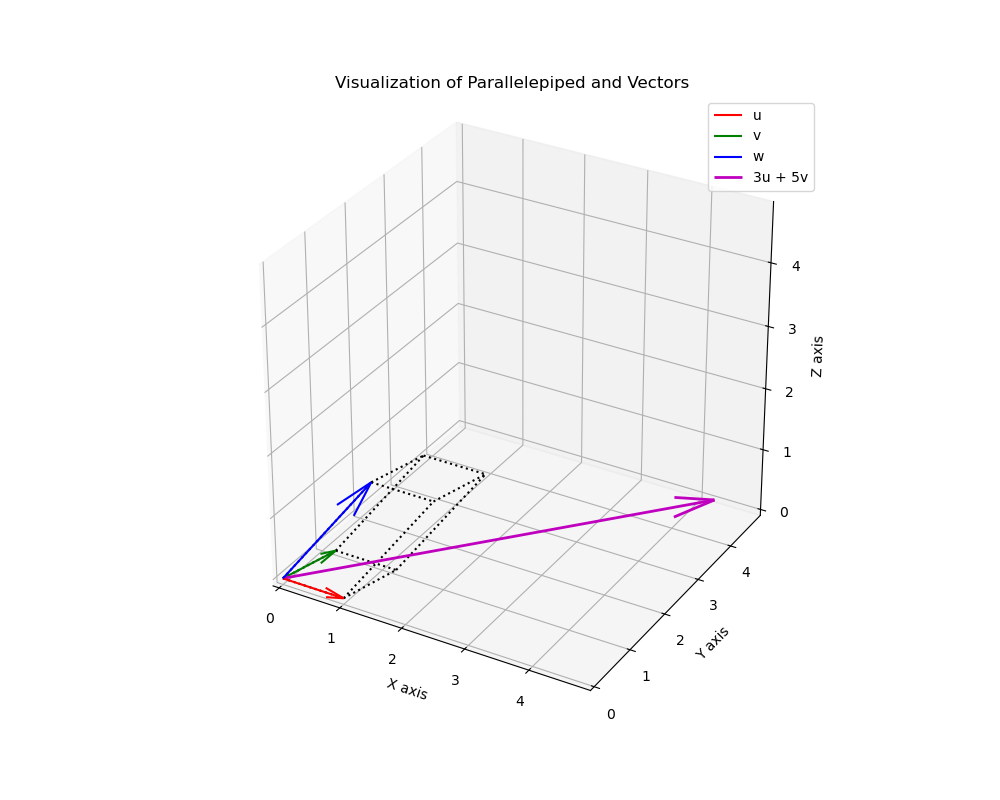
\includegraphics[width=1.1\columnwidth]{figs/2.10.82 2 .png}
    \caption{}
    \label{fig:placeholder}
\end{figure}
There appears to be a contradiction in the problem statement. The vectors $\vec{u}$ and $\vec{v}$ are given as **unit vectors**.Since the value of $\cos\theta$ must be in the range $[-1, 1]$, the given value $\vec{u}^\top\vec{v} = 4$ is impossible.

\end{document}